\chapter{Methods}

%\textbf{Tala um raunverulega ásæðu af hverju ég vel þessa íhluti!!!!!!}

\section{Hydrophone}\label{sec:AquarionHydro}

%\textbf{TALA UM AÐRA TÝPU SEM HEFÐI GETAÐ KOMIÐ TIL GREINA
%https://www.nauta-rcs.it/English/Instruments/Hydrophones/CetaceanResearchTech/C55/C55.html}

The first thing that needed to be determined was the hydrophone used.
Generally hydrophones are sensitive piezoelectric sensors that can detect small changes in pressure and convert that to an electrical signal.
This project will use the Aquarian audio H1a hydrophone, which was chosen for its low cost and good sensitivity, it was also readily available at the Reykjavik University lab.

\begin{table}[h]\caption{Important specifications of the Aquarian H1a hydrophone.\cite{noauthor_aquarian_nodate}}.\label{Tab:Aquarian}
\begin{tabular}{l|l}
Sensitivity     & -190dB re: 1V/µPa (+/- 4dB 20Hz-4KHz) \\\hline
Useful range    & \begin{tabular}[c]{@{}l@{}}100KHz (not measured above 100KHz, approximate sensitivity\\  @100KHz = -220dB re: 1V/µPa)\end{tabular} \\\hline
Capacitance     & 25nF \\ \hline
Operating depth & \textless{}80meters\\ \hline
Cost            &  159\$ \\ \hline
\end{tabular}
\end{table}

There is no preamplifier or impedance buffer circuit within the Aquarian H1a hydrophone, so the circuit needs to amplify the output signal of the hydrophone.
The gain of the circuit depends on what the intended use of the hydrophone will be.
In this case for cetaceans and large aquatic wildlife, Aquarian recommends gain of 40 - 50 dB and for very distant sounds 60dB.

\clearpage

\begin{equation}
    F_c = \frac{1}{ 0.000000157 R}  
\label{eq:fchydro}
\end{equation}

The Frequency response of the Aquarian H1a hydrophone can be calculated using \textit{Equation~\ref{eq:fchydro}} \cite{noauthor_aquarian_nodate}. 
Which is just \textit{Equation~\ref{eq:FC}} where the capacitance of the hydrophone has been multiplied with $2\pi$.


\subsection{Microcontroller og ADC}

\subsubsection{Microcontroller}
The Teensy3.5 was ultimately chosen for the microcontroller of the system.
This decision was made for several reasons.
The Teensy3.5 has two built-in ADC, which means the system might be able to add another hydrophone to it for recording.
Both ADCs have a maximum resolution of 16bits with a voltage range of 0 - 3.3V, or $\frac{3.3}{2^{16}} \approx 0.00005V \approx 50\mu V$ step size.
The Teensy also consumes little power, when running with no peripherals active the processor is powered roughly by 50mA at 5V or 0.25W.
Which is under the requirements set at the beginning of the project.
As well as it was readily available at the Reykjavik University lab.

\subsubsection{Operational amplifier}
%\textbf{Mögulega tala um í kafla 2 hvað mikilvægustu þáttir opampa fyrir þetta verkefni var}

The operational amplifier that was chosen for this project was the OPA1644 from Texas Instruments.
It was chosen its advertised superior sound quality and low noise spectral density of $\frac{5.1nV}{\sqrt{Hz}}$ at 1kHz.
%\begin{figure}[h]
%    \centering
%    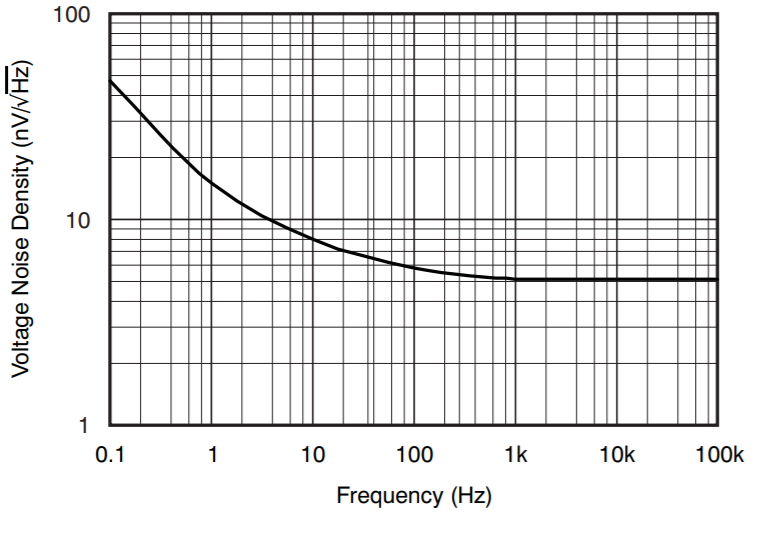
\includegraphics[width=0.7\textwidth]{graphics/noiseDensvsFreq.png}
%    \caption{\textbf{BÆTA}}
%    \label{fig:noiseDensvsFreq}
%\end{figure}
%Which means 
%https://www.designnews.com/what-nvvhz-noise
%\textbf{KYNNA Sér SNR}
%$$\sqrt{100*10^3Hz - 10Hz} = 3\sqrt{11110}Hz$$
%$$3\sqrt{11110}Hz*5.1*10^{-9}V = 1.6*10^{-6}V$$
%$$ 1.6*10^{-6}V * 100 = 1.6*10^{-4}$$
%Using a 1V output (0dBV) from the op amp the signal to noise ratio is:
%$$SNR = 20log_{10}(\frac{1V}{1.6*10^{-4}V}) \approx 76dB$$
It has low distortion of 0.00005\% at 1 kHz and a high slew rate of $\frac{20V}{\mu s}$.
As well as having a supply range that fits within the voltage range ($\pm2.25~-~\pm18$) of the Teensy analog pins of 3.3V\cite{noauthor_opa164x_nodate}.
It also has up to 40dB gain at 100kHz as seen in \textit{Figure~\ref{fig:dbvsFreq}}.

\begin{figure}[h]
    \centering
    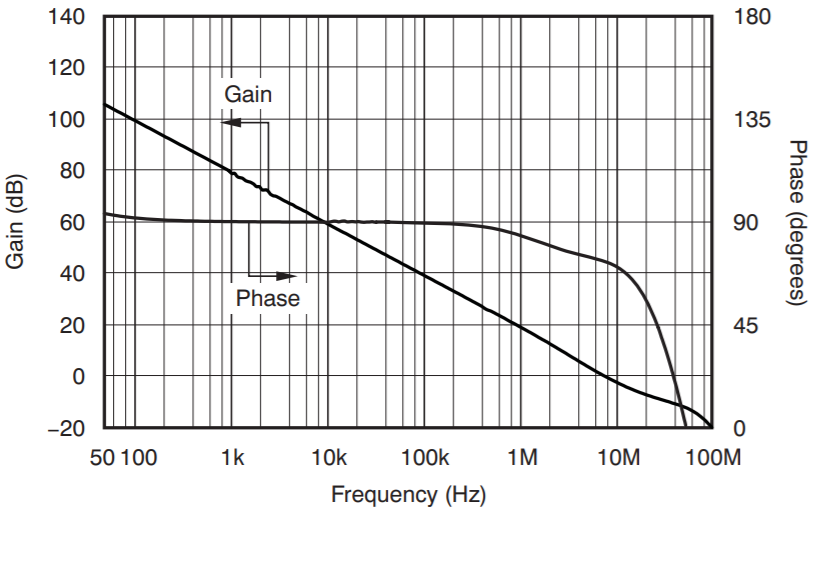
\includegraphics[width=0.7\textwidth]{graphics/dbVsfreq.png}
    \caption{Gain and phase shift vs frequency of the OPA1644\cite{noauthor_opa164x_nodate}}
    \label{fig:dbvsFreq}
\end{figure}


\vspace{4cm}


\section{Circuit}\label{sec:CircResult}

%From the project goals the circuit needs to be able to gather data from signals with frequencies between 10 - 100kHz. 
It was decided to collect signals ranging from 10 - 100kHz, the lower limit which was chosen after seeing \textit{Table~\ref{Tab:WhaleHz}} and the dominant frequencies, the higher limit was chosen because the project goal was to maximize the absolute limits of the device.
This could be significantly reduced since most dominant frequencies are lower than 30kHz however, there are vocalization that goes up to and over 100kHz so it is interesting to see if the Teensy was capable of recording these high-frequency signals.
The Aquarian H1a hydrophone datasheet specifies that for cetacean vocalization recording the gain of the preamplifier needs to be between 40 - 50 dB\cite{noauthor_aquarian_nodate}.
The circuit will there for consist of an active low pass filter and high pass filter, a scaling summing amplifier and an inverting op-amp.
It will then connect to the Teensy 3.5 built-in ADC.\\
\indent \textit{Figure \ref{fig:Opamp1}} shows the first part of the circuit.
The output of the hydrophone is first connected to a high pass filter, where the capacitance, 25nF of the hydrophone is used as the capacitor in the high pass filter.

\begin{figure}[h]
    \centering
    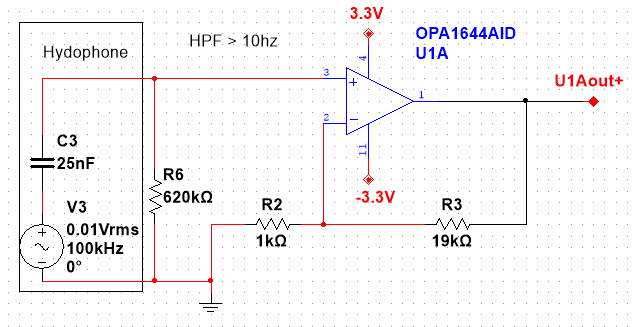
\includegraphics[width=0.70\textwidth]{graphics/OPamp1.png}
    \caption{The first part of the circuit where the output of the hydrophone first filtered using an active high pass filter and then connected to a operational amplifier and amplifying the signal by 20.}
    \label{fig:Opamp1}
\end{figure}

\vspace{4cm}

The desired value for the high pass filter was 10Hz and using \textit{Equation~\ref{eq:fchydro}} provided in the datasheet, the resistor value was estimated.   
$$F_c = \frac{1}{2\pi * 25nF * 636k\Omega} = 10Hz$$
Using standard resistor values, the closest resistor value is 620k which yields a cut off frequency of 10.26Hz.
The gain over the active high pass filter can be represented using \textit{Equation \ref{eq:DCGain}} and \textit{Equation \ref{eq:ActiveHighPass}}. 
Where $A_{V1} = 1 + \frac{19k\Omega}{1k\Omega} = 20$.
$$A_f = \frac{(1+\frac{19k}{1k})(\frac{f}{10.26Hz})}{\sqrt{1 + (\frac{f}{10.26Hz})^2}} \approx 20$$
Which is approximately equal to 20, as seen in \textit{Figure~\ref{fig:AVhighpass}} over the entire bandwidth.

\begin{figure}[h]
    \centering
    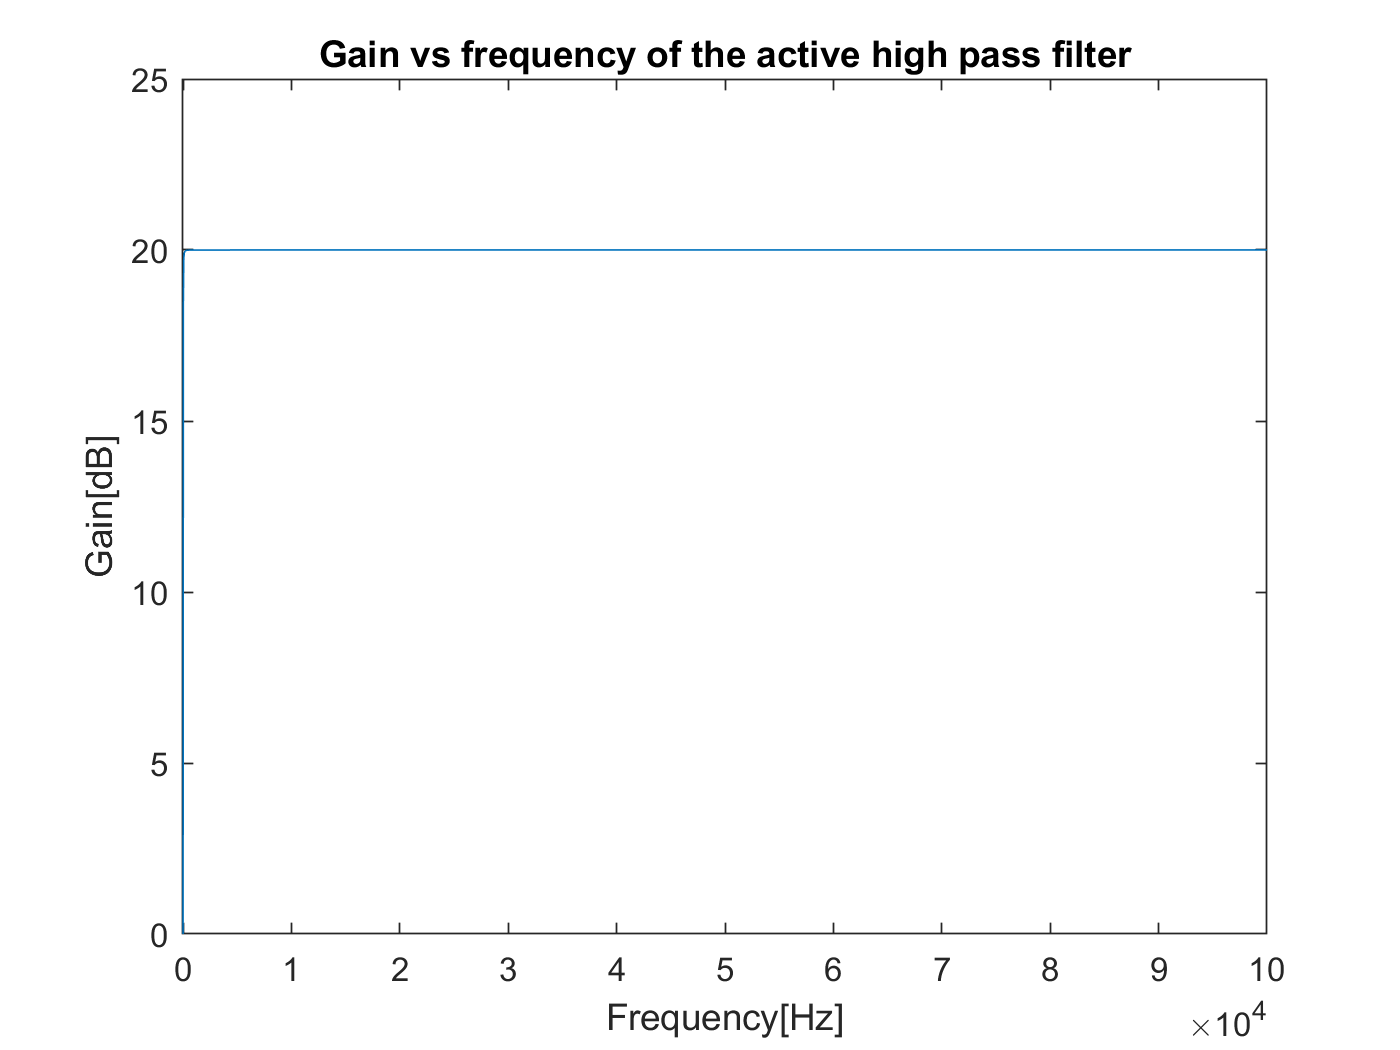
\includegraphics[width=0.5\textwidth]{graphics/Av_Highpass.png}
    \caption{The gain of the operational amplifier with the active high pass filter.}
    \label{fig:AVhighpass}
\end{figure}

\vspace{4cm}

\textit{Figure \ref{fig:Opamp2}} shows the active low pass filter configuration which has a cut-off frequency of $\approx$ 100kHz and a gain of 2.5.

\begin{figure}[h]
    \centering
    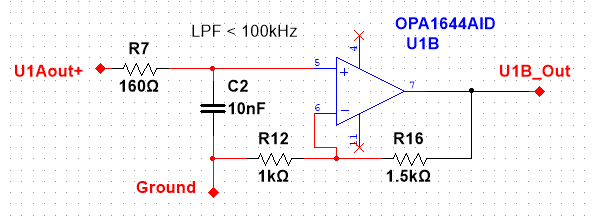
\includegraphics[width=0.7\textwidth]{graphics/OPamp2.png}
    \caption{The second operational amplifier, where the signal is first filtered by the active low pass filter as well as amplifying the signal.}
    \label{fig:Opamp2}
\end{figure}

The desired value for the high pass filter was 100kHz and using \textit{Equation~\ref{eq:FC}} and choosing a resistor value of 160$\Omega$, the capacitor value was estimated.   
$$F_c = \frac{1}{2\pi 9.9nF 160\Omega} = 100kHz$$
Using standard capacitor values, the closest capacitor value is 10nF which yields a cut off frequency of 99472Hz.
The gain over the active low pass filter can be represented using \textit{Equation \ref{eq:DCGain}} and \textit{Equation \ref{eq:ActiveLowPass}}. 
Where $A_{V1} = 1 + \frac{1.5k\Omega}{1k\Omega} = 2.5$.
$$A_f  = \frac{1 + \frac{1.5k\Omega}{1k\Omega}}{\sqrt{1 + (\frac{f}{99471.8Hz})^2}}$$
Which is approximately equal to 2.5 over the entire bandwidth. 
\textit{Figure~\ref{fig:AVlowpass}}.

\begin{figure}[h]
    \centering
    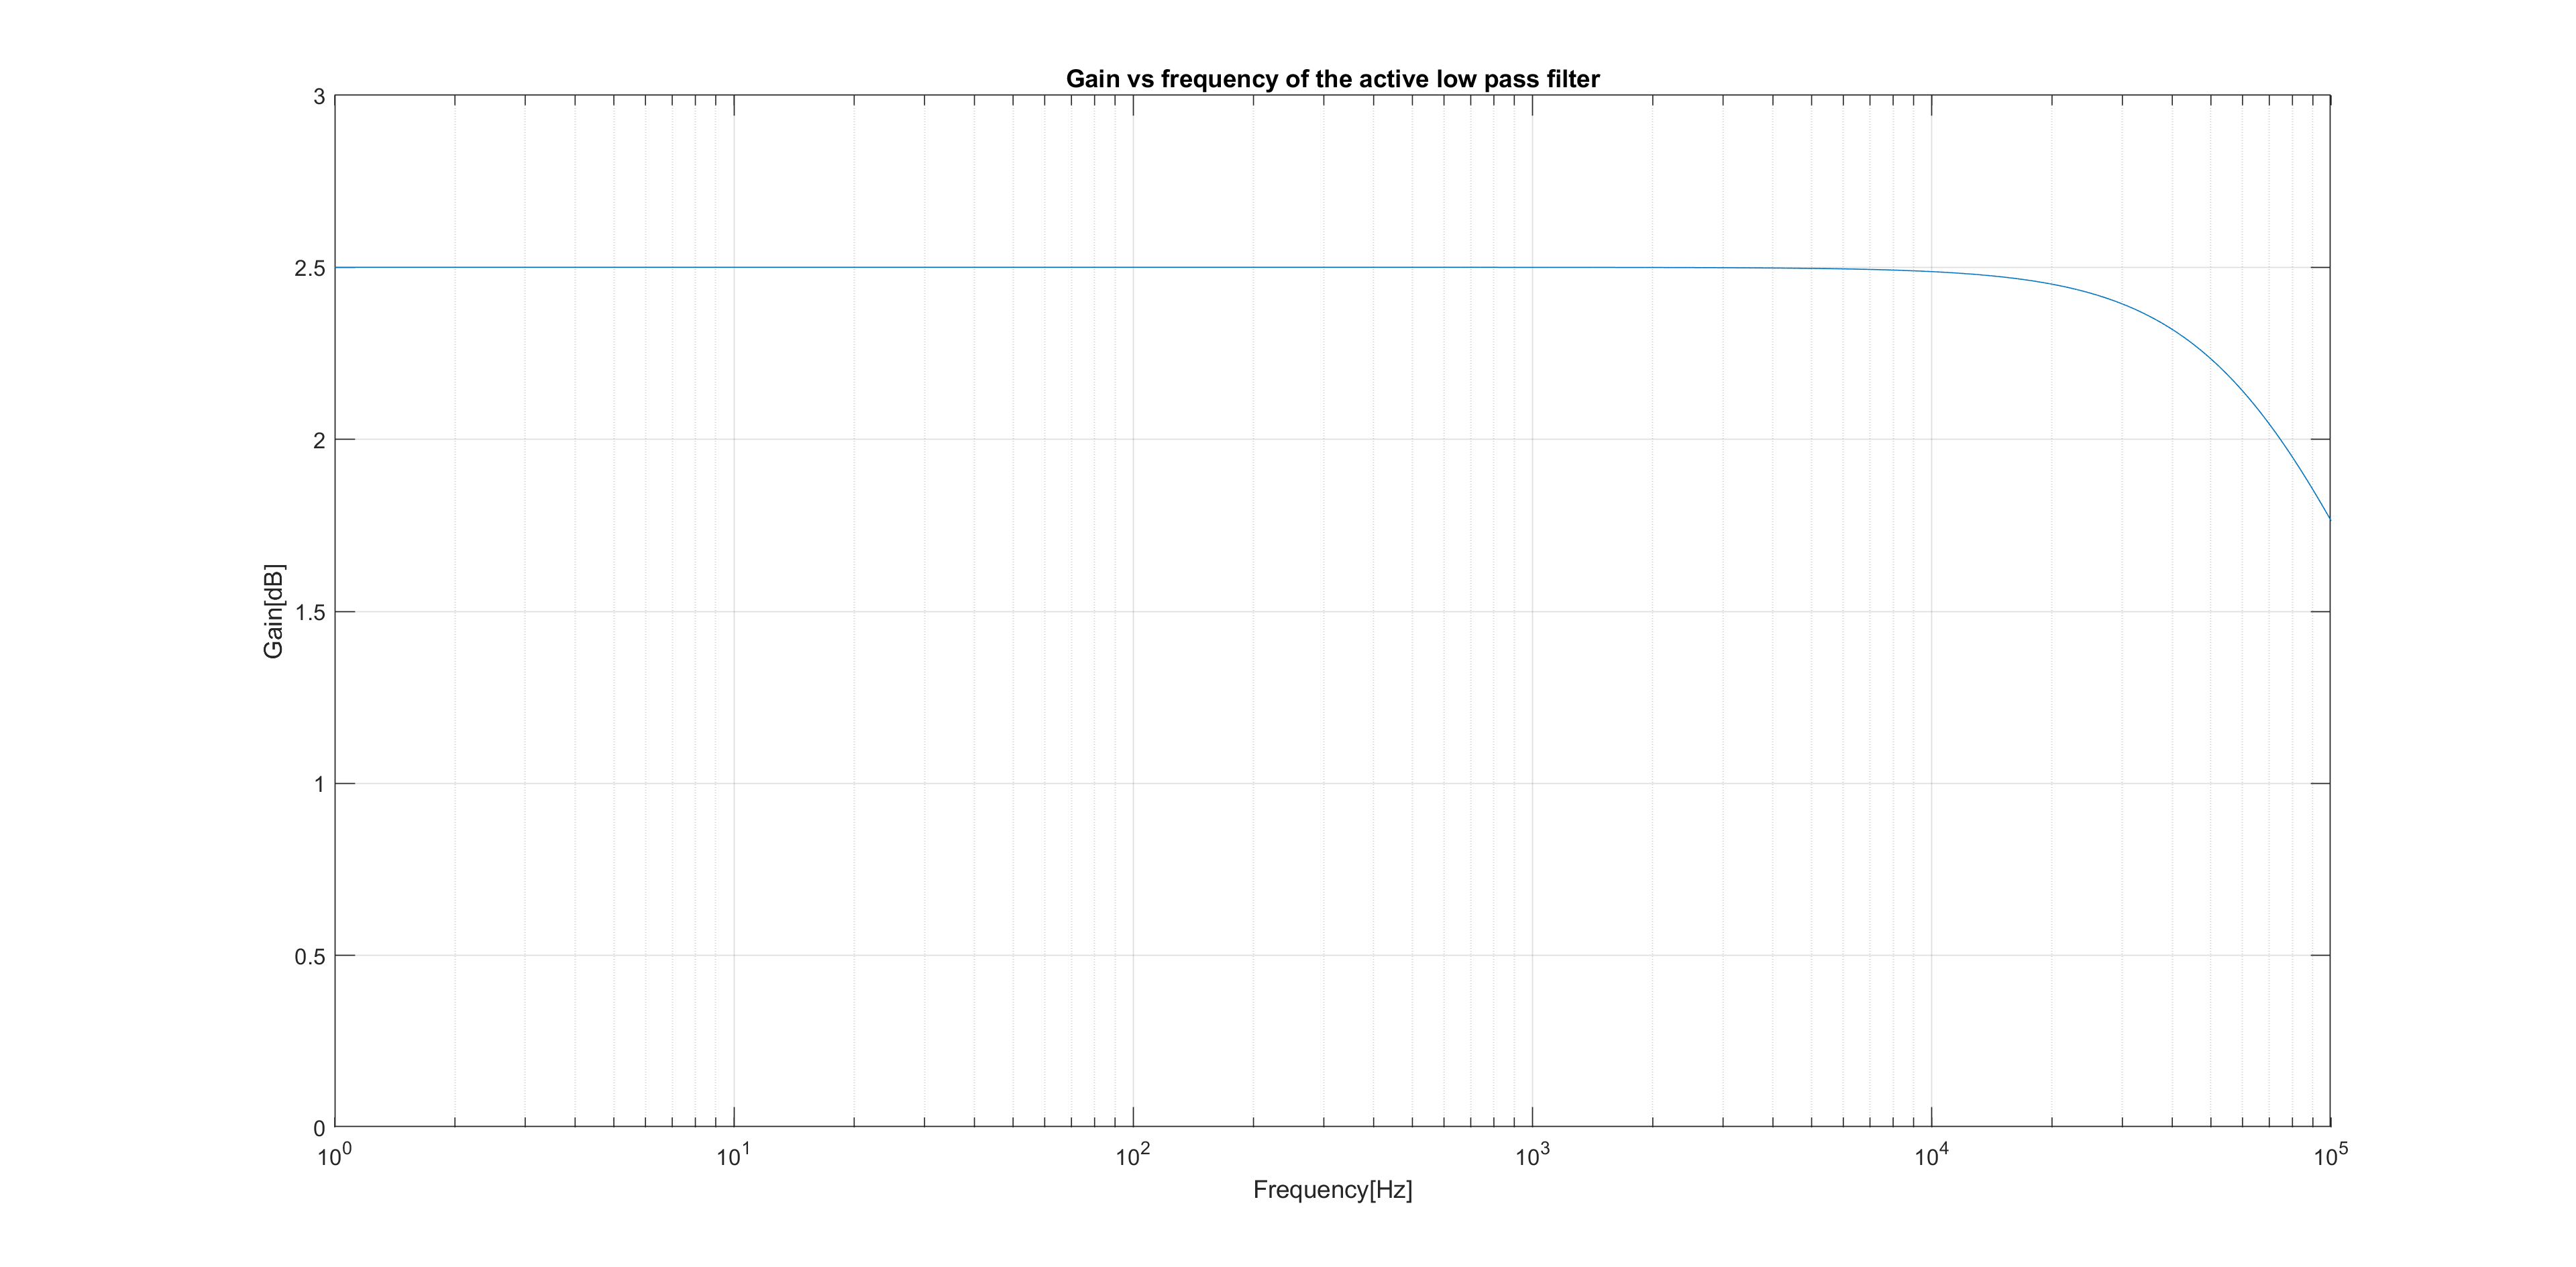
\includegraphics[width=0.6\textwidth]{graphics/Av_Lowpass.png}
    \caption{The gain of the operational amplifier with the active low pass filter.}
    \label{fig:AVlowpass}
\end{figure}

\textit{Figure~\ref{fig:Opamp3}} shows the scaling summing operational amplifier which is used to shift the input signal by 1.65Vdc. 


\begin{figure}[h]
    \centering
    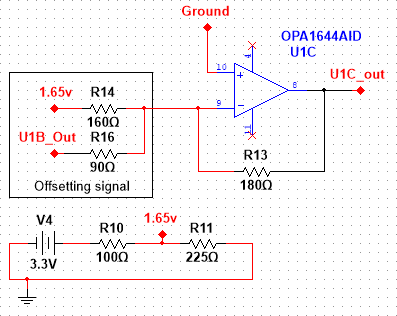
\includegraphics[width=0.70\textwidth]{graphics/OPamp3.png}
    \caption{The scaling summing operational amplifier, where the signal is shifted by 1.65Vdc}
    \label{fig:Opamp3}
\end{figure}


Which is important since the analog pins of the Teensy 3.5 have a voltage range of 0-3.3V.
There for the signal needs to be shifted by 3.3V/2 = 1.65Vdc.
%To estimate the voltage output of the op amplifier, \textit{Equation \ref{eq:invertDCGain}} and \textit{Equation \ref{eq:ScalingGain}} was used.
%For an input signal of 10mV amplitude, of the scaling summing op amp would be \textbf{KANSKI EKKI HAFA ?!?!?!} 
%$$V_{out} = -180\Omega(\frac{1.65V}{180\Omega} + \frac{\pm 10mV}{90\Omega}) = \pm $$
A voltage divider was needed to determine the resistor values for the 1.65Vdc which would ultimately put some design restraints on R16 and R13 seen in \textit{Figure~\ref{fig:Opamp3}}.
Firstly it was decided to have $R10 = 100\Omega$  and $R11 = 225\Omega$ to start off the calculations.
From that R14 could be calculated as $180\Omega$.
$$3.3V = \frac{\frac{1}{\frac{1}{180\Omega}+\frac{1}{225\Omega}}}{100\Omega+\frac{1}{\frac{1}{180\Omega}+\frac{1}{225\Omega}}} = 1.65V$$
Which was changed to $160\Omega$ because of the addition of R16 and using Multisim it was determined that $160\Omega$ would yield the closest results to the 1.65Vdc.
The gain for the input signal from the low pass filter is found by using \textit{Equation \ref{eq:invertDCGain}}
$$A_{V3} = -\frac{180\Omega}{90\Omega} = -2$$
The operational amplifier is in an inverting configuration which turns positive voltage signals to negative.
This needs to be rectified since the Teensy 3.5 analog pins do not have a negative voltage range.
Which is done by another inverting operational amplifier the output of which connects to the A9 analog pin on the Teensy via a 330$\Omega$ resistor which limits the current to under 100mA, seen in \textit{Figure~\ref{fig:Opamp4}}.

\begin{figure}[h]
    \centering
    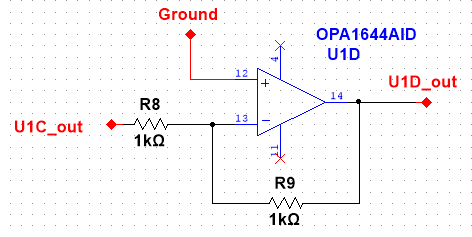
\includegraphics[width=0.70\textwidth]{graphics/OPamp4.png}
    \caption{The final operational amplifier, which is in an inverting configuration.}
    \label{fig:Opamp4}
\end{figure}

The gain of inverting amplifier is found using \textit{Equation \ref{eq:invertDCGain}}.
$$ A_{V4} = -\frac{1k \Omega}{1k \Omega} = -1$$
%The total circuit therefore consists of four operational amplifiers, high pass and low pass filter.
%\textbf{MÖGULEGA BÆTA JÖFNU 'I KAFLA 2}
The total gain of the circuit for the input signal is found by.

$$A_{tot} = A_1A_1A_2A_3A_4 = 20*2.5*-2*-1 = 100$$

Finding the total dB gain of the circuit can be found by \textit{Equation \ref{eq:DBGAIN}}, which is confirmed using Multisim as seen in \textit{Figure~\ref{fig:bode}}.

$$dB = 20log(100) = 40dB$$


\begin{figure}[h]
    \centering
    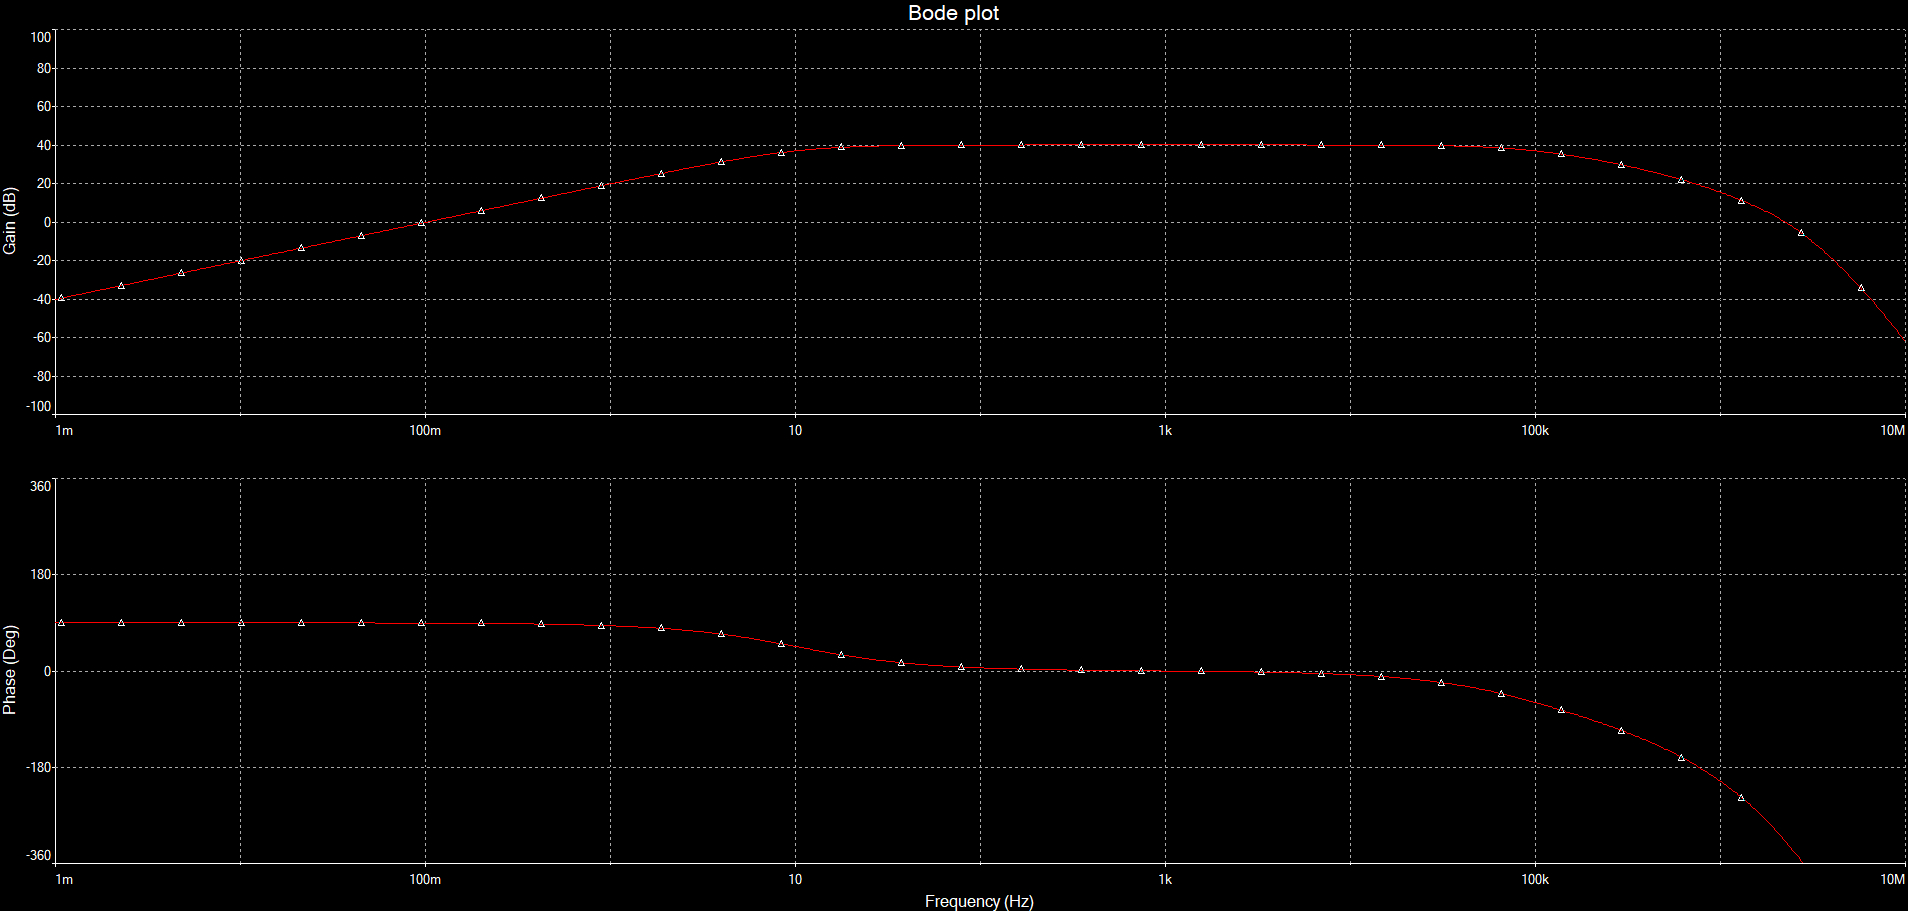
\includegraphics[width=1.0\textwidth]{graphics/bodeNew.png}
    \caption{The bode plot of the circuit.}
    \label{fig:bode}
\end{figure}

The bode plot of the circuit can be seen in \textit{Figure~\ref{fig:bode}}.
It shows the circuit has a dB gain of $\approx$ 40, for the entire bandwidth of 10 - 100kHz.



%Several simulations of the circuit were performed in Multisim.
%Which yielded the results seen in \textit{Figure~\ref{fig:InpVsOut10} -~\ref{fig:bode}}.
%Using the setup of the circuit seen in \textit{Figures~\ref{fig:Opamp1}~\ref{fig:Opamp2}~\ref{fig:Opamp3}~\ref{fig:Opamp4}}. 
%\textbf{LAGA MYNDIR EFTIR testinu}

%\begin{figure}[h]
%    \centering
%    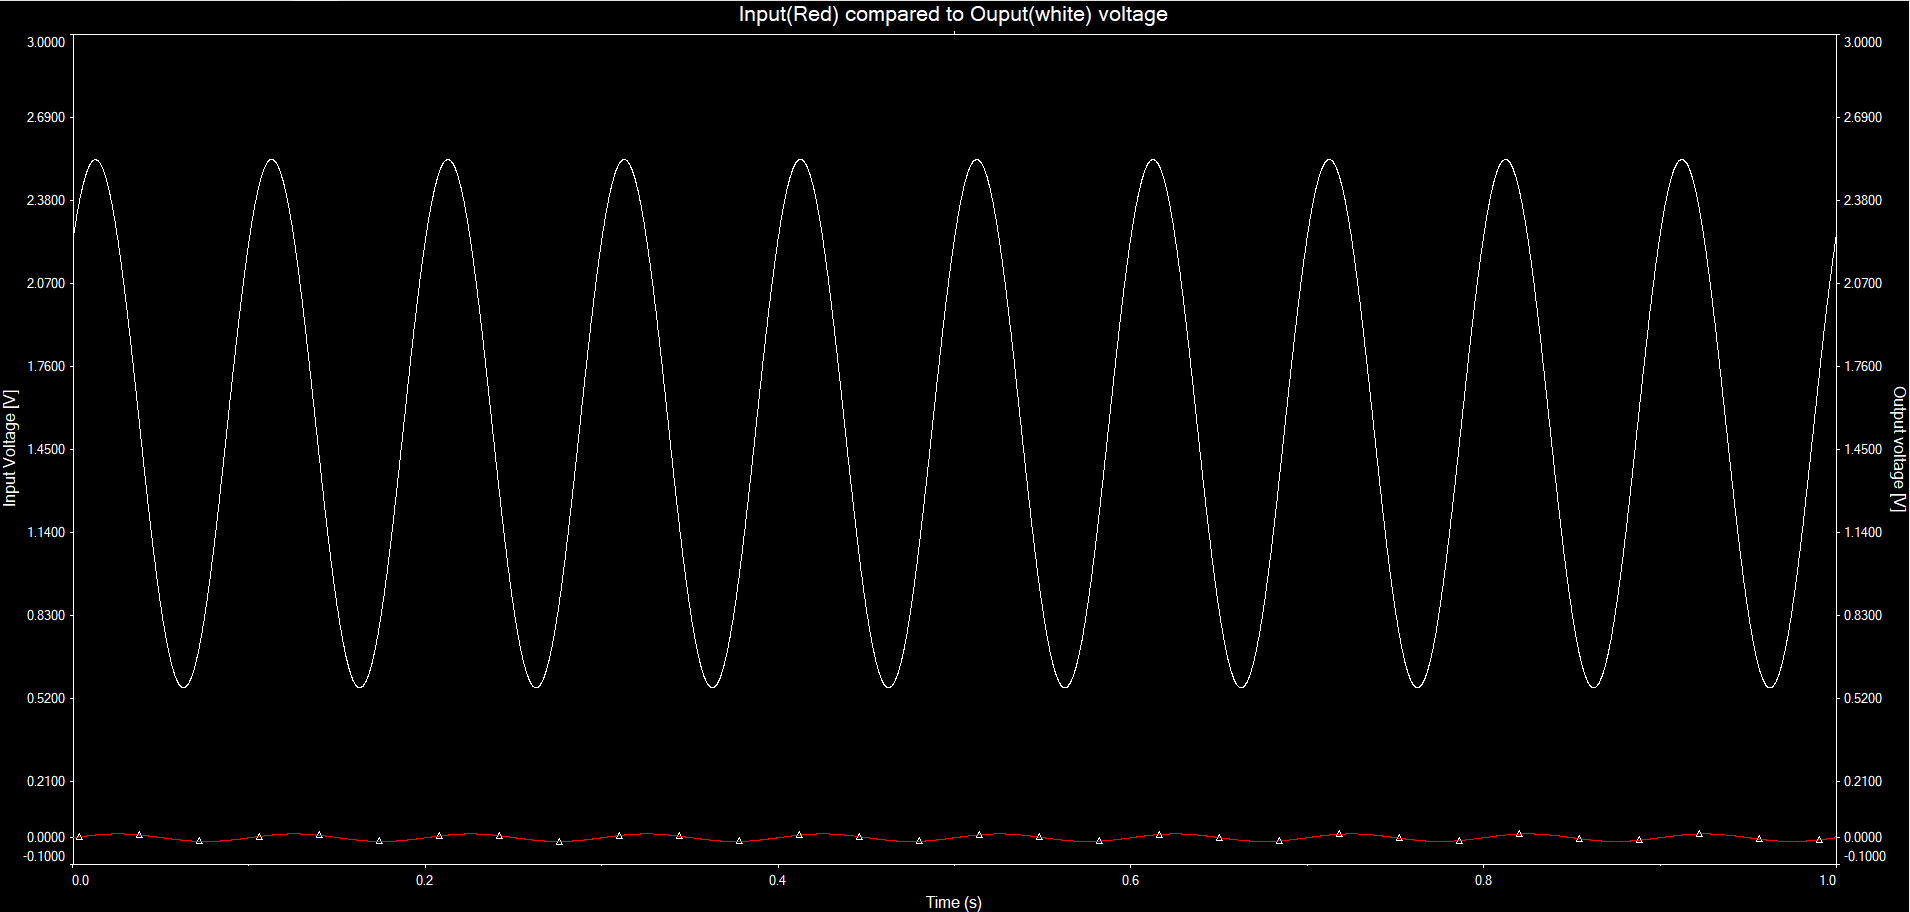
\includegraphics[width=1.0\textwidth]{graphics/InpVsOut10hz.png}
%    \caption{With an input signal of 10mV RMS, at 10HZ.}
%    \label{fig:InpVsOut10}
%\end{figure}

%The simulation was run using an AC voltage generator which was set to output 10mV RMS and 10Hz.
%Which yielded the results seen in \textit{Figure~\ref{fig:InpVsOut10}}.
%\textbf{TALA UM MEIRA}

%\begin{figure}[h]
%    \centering
%    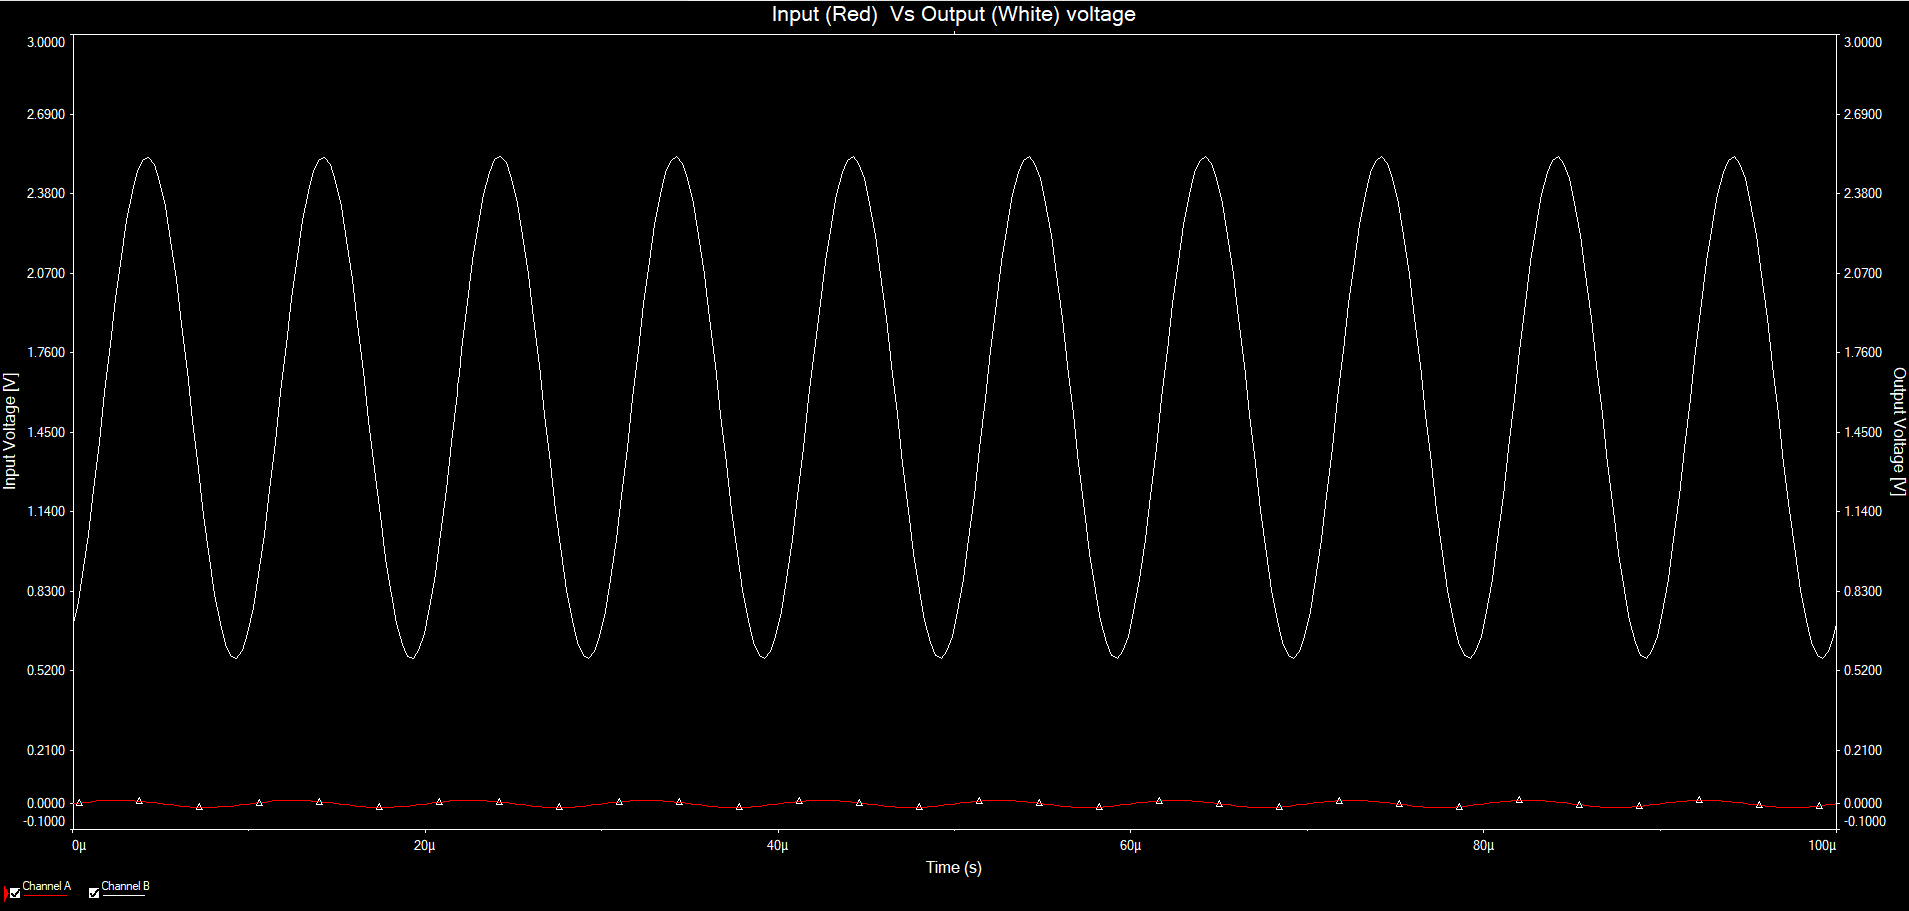
\includegraphics[width=1.0\textwidth]{graphics/InpVsOut100khz.png}
%    \caption{With an input signal of 10mV RMS, at 100kHZ.}
%    \label{fig:InpVsOut100k}
%\end{figure}

%\textbf{Bæta VIÐ 50khz multisim testi}

%The simulation was run using an AC voltage generator which was set to output 10mV RMS and 100kHz.
%Which yielded the results seen in \textit{Figure~\ref{fig:InpVsOut100k}}.
%\textbf{TALA UM MEIRA}

\clearpage

\subsection{Direct memory access}

When transferring data between main memories and I/O devices, direct memory access (DMA) can be utilized.
The benefit of using DMA for the data transfer is that it minimizes or eliminates the processor's involvement with the data transfer.
The processor only initializes the DMA controller by configuring the read and write memory, size of data for each transfer and I/O address.
In \textit{Figure~\ref{fig:DMAcontroller}} the process of the data transfer is better explained.

\begin{figure}[h]
    \centering
    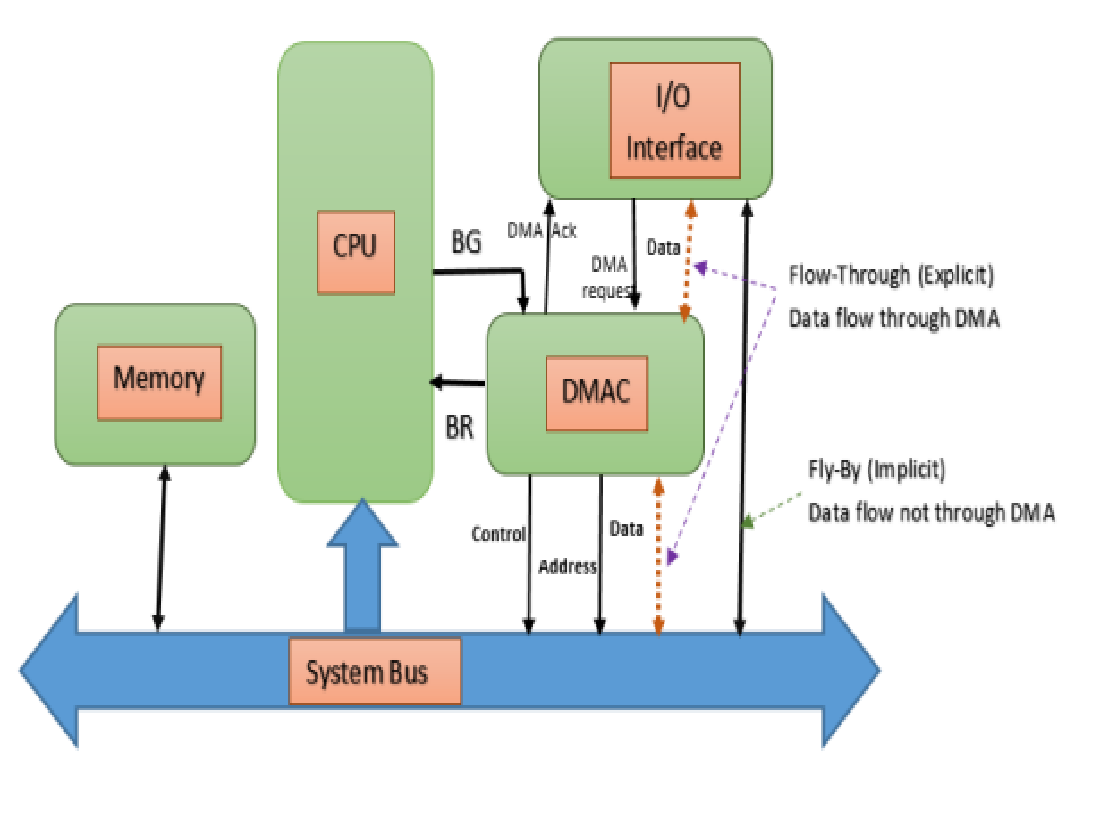
\includegraphics[width=0.70\textwidth]{graphics/DMA.png}
    \caption{Data transfer for a DMA controller. Where the data transfers from the I/O device directly to memory. \cite{ahmed_design_2019}}
    \label{fig:DMAcontroller}
\end{figure}

A bus request (BR) signal is sent to the processor during the data transfer operation.
The processor then finishes its current job and replies with a bus grant (BG) signal.
The DMA controller receives the signal and can then initiate the data transfer.
There are two modes in which the DMA can perform data transfers.
The first is called flow-through, where the data flows through the DMA controller between the I/O device to memory.
The second is called fly by, where the data is transferred directly between the I/O device and memory \cite{ahmed_design_2019}.


%%% Local Variables: 
%%% mode: latex
%%% TeX-master: "DEGREE-NAME-YEAR"
%%% End: 
